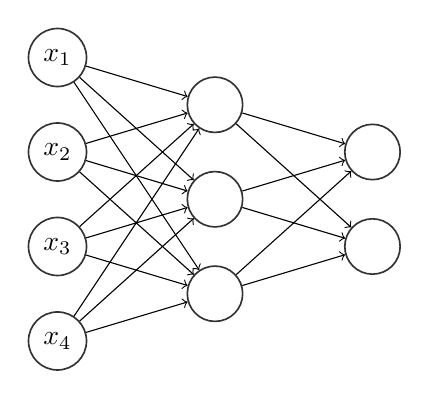
\begin{tikzpicture}
	\tikzstyle{neuron} = [circle,draw=black!80,semithick,minimum size=20pt]
	% input layer
	\foreach \i in {1,...,4}
		\node[neuron] (input\i) at (0, -\i*1.2) {$x_\i$};
	% hidden layer
	\foreach \i in {1,...,3}
		\node[neuron] (hidden\i) at (2, -\i*1.2 -.6) {};
	% output layer
	\foreach \i in {1,...,2}
		\node[neuron] (output\i) at (4, -\i*1.2 -1.2) {};
	% connections input->hidden
	\foreach \i in {1,...,4}
		\foreach \j in {1,...,3}
			\draw[->] (input\i) -- (hidden\j);
	% connections hidden->output
	\foreach \i in {1,...,3}
		\foreach \j in {1,...,2}
			\draw[->] (hidden\i) -- (output\j);
\end{tikzpicture}